% file: manual.tex
% author: Jiri Kristof, xkrist22
% FIT VUT ISA project - dns resolver
% documentation

\documentclass[a4paper, 11pt]{article}


\usepackage[czech]{babel}
\usepackage[utf8]{inputenc}
\usepackage[left=2cm, top=3cm, text={17cm, 24cm}]{geometry}
\usepackage{times}
\usepackage{graphicx}
\usepackage[unicode]{hyperref}
\hypersetup{
	colorlinks = true,
	hypertexnames = false,
	citecolor = red
}

\begin{document}
	\begin{titlepage}
		\begin{center}
			
\includegraphics[width=0.77\linewidth]{FIT_logo.pdf} \\

			\vspace{\stretch{0.382}}

			\Huge{Projektová dokumentace} \\
			\LARGE{\textbf{
				DNS resolver
			}} \\
			\Large{Síťové aplikace a~správa sítí}

			\vspace{\stretch{0.618}}
		\end{center}

		{\Large
			\today
			\hfill
			Jiří Křištof (xkrist22)
		}
	\end{titlepage}
	
	\setcounter{tocdepth}{1}
	\thispagestyle{empty}
	\tableofcontents
	\clearpage
	
	\pagenumbering{arabic}
	\setcounter{page}{1}

	\section{Úvod}
	Cílem projektu je vytvořit aplikaci DNS resolver v~jazyce \texttt{C/C++}. Program naslouchá na vybraném portu~a filtruje DNS dotazy. DNS resolver podporuje dotazy typu~A zaslané pomocí UDP protokolu transportní vrstvy. Pro ostatní dotazy je zaslán DNS paket informující o problému.
	Resolver načte~z dodaného souboru domény určené~k vyfiltrování. Pokud je~v dotazu požadován překlad doménového jména, či jeho subdomény, který je uveden ve filtru, pak je tento dotaz zahozen.~V opačném případě je dotaz dále přeposlán na specifikovaný DNS server~a zpráva z~něj je vrácena původnímu tazateli.

	\section{Teoretický základ}
	DNS je protokol aplikační vrstvy modelu TCP/IP. Jedním z využití DNS je překlad doménových jmen na IP adresy, který je pro tento projekt stěžejní. Při DNS komunikaci je na transportní vrstvě využívána komunikace pomocí UDP datagramů. 
	
	\subsection{DNS rezoluce}
	Rezoluce je proces hledání odpovědi v systému DNS. DNS prohledává strom, v kterém jsou uloženy záznamy obsahující doménové jméno a k němu odpovídající adresu. Rezoluce může být buď rekurzivní, nebo iterativní.
	
	V případě rekurzivního dotazu je tazateli ze serveru vrácena odpověď a dohledávání uloženého záznamu je plně na DNS serveru. Ten, pokud nemá uložen požadovaný záznam, se musí na tento záznam sám doptat jiných DNS serverů.
	
	V případě iterativního dotazu vrací DNS server buď odpověď na dotaz -- přeložené doménové jméno, nebo adresu jiného DNS serveru, který odpověď zná, nebo jí je \uv{blíže}. 
	
	\subsection{DNS paket}
	DNS paket se skládá z 5 částí uvedených v obrázku \ref{fig:1}. V rámci projektu jsou důležité první 3 části -- hlavička, dotaz a odpověď. 
	\begin{figure}[h]
		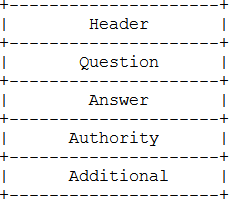
\includegraphics[width=4cm]{dnspacket.png}
		\centering
		\caption{Struktura DNS paketu}
		\label{fig:1}
	\end{figure}

	\newpage

	\subsubsection{Hlavička}
	Hlavička obsahuje informace o paketu -- jeho identifikační číslo, příznaky, počty informací v dalších částech nebo návratové a operační kódy. Struktura hlavičky DNS paketu je popsána na obrázku \ref{fig:2}.

	\begin{figure}[h]
		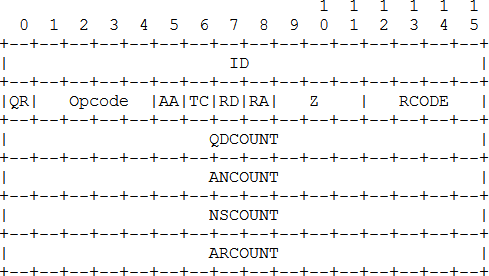
\includegraphics[width=7cm]{dnsheader.png}
		\centering
		\caption{Struktura hlavičky DNS paketu}
		\label{fig:2}
	\end{figure}
	
	Každá položka hlavičky udává určité informace o celém paketu:

	\begin{itemize}
	\item \texttt{ID}: identifikátor paketu.
	\item \texttt{QR}: příznak, který je nastaven do hodnoty 1 v případě, že paket představuje odpověď, jinak obsahuje hodnotu 0.
	\item \texttt{OpCode}: operační kód specifikující typ paketu, v rámci projektu není podstatný.
	\item \texttt{AA}: příznak nastavený do hodnoty 1, pokud odpověď pochází z autoritativního DNS serveru
	\item \texttt{TC}: Detekce zkrácené odpovědi, v rámci projektu není jeho význam důležitý.
	\item \texttt{RD}: bit je nastaven do hodnoty 1, pokud klient vyžaduje použití rekurzivní rezoluce.
	\item \texttt{RA}: bit nastavuje DNS server, pokud vyhoví požadavku klienta na rekurzivní rezoluci.
	\item \texttt{Z}: bity rezervované pro budoucí využití, jsou vždy nastaveny na hodnotu 0.
	\item \texttt{RCode}: kód specifikující chyby. Bližší popis a jejich využití v projektu je uveden v tabulce \ref{tab:2}.
	\end{itemize}

	Dále hlavička DNS paketu obsahuje počty dotazů a počty v dalších sekcích paketu. DNS resolver kontroluje počet dotazů uvedený v \texttt{QDCOUNT} části DNS hlavičky.

	\subsubsection{Dotaz}
	Tělo DNS zprávy se skládá z dotazů, ke kterým je uveden typ a třída. DNS resolver podporuje pouze 1 dotaz v těle zprávy, pro jiný počet zpráv je zaslán chybový DNS paket s kódem 4 -- požadovaná služba není implementována.

	\section{Návrh a implementace}
	Aplikace je rozdělena do jednotlivých souborů obsahující implementaci tříd, které implementují výsledný systém. Zdrojové soubory se nachází v adresáři \texttt{src}.
	
	Po spuštění programu jsou zpracovány argumenty předané z příkazové řádky. Poté je spuštěn server, který vytváří filtr a čeká na DNS pakety na uvedeném portu.
	
	\subsection{Parsování vstupních argumentů}
	Parsování vstupních argumentů předané programu~z příkazového řádku zajišťuje třída \texttt{argparse}. Při vytváření instance třídy jsou konstruktoru předány veškeré parametry~z příkazové řádky. Po zpracování je možné se pomocí~k tomu určených metod dotazovat na potřebné údaje -- IP adresu dns serveru, jméno souboru obsahující filtr~a případně číslo portu. 
	
	V případě, že je programu předáno doménové jméno dns serveru, pak je jeho IP adresa dohledána pomocí funkce \texttt{gethostbyname}. 
	
	Neplatné vstupní argumenty jsou ignorovány. V případě, že je programu zadáno neplatné číslo portu, pak program využije výchozí hodnotu 53. Program končí v chybovém stavu, pokud nezíská informaci o IP adrese dns serveru a název souboru obsahující filtr. 
	
	
	Aplikace může být přepnuta do módu, v němž je uživatel informován o jednotlivých krocích programu zprávami směřovanými na standardní výstup. Mód může být aktivován využitím přepínače \texttt{-v}. Výpis informací je implementován třídou \texttt{verbose}.

	\subsection{Zpracování souboru filtru}
	Zpracování vstupního souboru obsahující filtr je implementováno třídou \texttt{filter}. Při vytváření objektu třídy je konstruktoru předán název souboru obsahující filtr. Konstruktor ukládá jednotlivé řádky obsahující doménová jména k vyfiltrování do vektoru textových řetězců. 
	
	Při zpracovávání souboru jsou vynechány prázdné řádky a řádkové komentáře začínající symbolem \texttt{\#}. Před zpracováváním každého řádku je prvně provedeno odebrání bílých znaků na začátku a na konci daného řádku.
	
	V případě, že soubor neexistuje, je program ukončen a na standardní chybový výstup je uvedena informace o nastalé chybě. 
	
	\subsection{Serverová část}
	Zajištění síťové komunikace s klientem zasílající DNS dotazy je implementováno pomocí třídy \texttt{server}. Konstruktoru objektu třídy server jsou předány hodnoty čísla portu, na němž má server čekat na zprávy, ip adresa dns serveru, na nějž mají být směrovány dotazy, které nebudou vyfiltrovány, a jméno souboru obsahující domény určené k vyfiltrování.
	
	Po extrakci dat z filtru je vytvořen soket serveru, který je napojen na daný port. V případě problémů s vytvářením soketu a jeho připojením na port je program ukončen s příslušným chybovým kódem a na standardní chybový výstup je vypsána hláška vysvětlující důvod ukončení programu.

	Po vytvoření instance třídy \texttt{server} je možné spustit pomocí metody \texttt{run\_server} samotný server, který čeká na dns dotazy, které buď vyfiltruje a zašle paket s příslušným návratovým kódem, nebo paket přeposílá dál. 
	
	V případě chyby na straně serveru je klientovi zaslán DNS paket informující o selhání serveru. Pokud server detekuje při příjmu, zpracovávání, nebo odesílání paketu problém, pak ukončuje zpracovávání daného paketu a čeká na příchod dalšího. Pokud je server spuštěn pomocí metody \texttt{run\_server}, pak je jej možné ukončit pouze vysláním příslušného signálu, např. \texttt{SIGINT}.
	
	\subsection{Klientská část}	
	Komunikaci s určeným DNS serverem je implementována pomocí třídy \texttt{client}. Při instanciaci je vytvořen soket, který je připojen na port 53, jenž je primárně určen pro DNS komunikaci. 
	
	Pomocí soketu je možné zaslat s využitím funkce \texttt{send\_data} DNS paket dále DNS serveru, který tento přeloží a zašle zpět. Přijatý paket je poté vrácen tazateli, tedy objektu třídy \texttt{server}. 
	
	Metoda zasílající data vrací DNS odpověď a délku vráceného paketu. Soket je možné zavřít pomocí metody \texttt{close\_socket}. Při zpracovávání jednoho DNS paketu je postupně otevřen soket, zaslány data a soket poté uzavřen. Při zpracovávání dalšího paketu je tento proces opakován.
	
	\subsection{Módy aplikace}
	Aplikace může pracovat ve dvou různých režimech. Ve výchozím nastavení pracuje server v tichém režimu -- na standardní výstup nejsou vypisovány žádné informace, případné chybové hlášky jsou vypisovány na standardní chybový výstup. Výpisy jsou realizovány pomocí k tomu určených třídních metod třídy \texttt{verbose}. 
	
	Hlášení průběhu překladu jsou uvozena znakem \texttt{*} a je možné je tak odlišit od hlášek směřovaných na standardní chybový výstup.
	
	\subsection{Chybové stavy}
	Pokud se program dostane do chybového stavu, pak tento stav řeší třídní metody třídy \texttt{err\_handler}. Třída informuje uživatele o problému. Pokud nelze dále pokračovat a chybový stav ošetřit, pak je program ukončen s chybovým návratovým kódem. Chybové kódy jsou uvedeny v tabulce \ref{tab:1}.
	
	Chybová hlášení jsou vypisována na standardní chybový výpis. Pro jednodušší odlišení od výpisu na standardní výstup jsou tato hlášení uvozena znaky \texttt{***}.
	
	\subsection{Pomocné funkce}
	V rámci projektu jsou využívány další pomocné metody implementované třídou \texttt{func}. Pomocí regulárních výrazů jsou validovány IP adresy předané jako argument z příkazové řádky. Je tak možné detekovat chybu dříve, než je tato adresa využita pro vytvoření soketu připojující se na DNS server. 
	
	Další funkce umožňují zkontrolovat, zda uvedený textový řetězec obsahuje pouze čísla -- je možná kontrola čísla portu. Při zpracovávání souboru obsahující filtr jsou pak využívány metody odebírající bílé znaky ze začátku a konce textového řetězce. 
	
	\section{Překladový systém}
	Překladový systém je vytvořen pomocí utility \texttt{make}. Zdrojové soubory je možné přeložit pomocí připojeného souboru \texttt{Makefile}. Pro překlad je využíván kompilátor \texttt{gcc}. Po překladu je v kořenovém adresáři projektu umístěn spustitelný soubor \texttt{dns}.
	
	Pomocí příkazu \texttt{make test} je možné spustit testy, které byly využity při testování aplikace. 
	
	\section{Návod na použití}
	Po stažení zdrojových souborů proveďte překlad pomocí utility \texttt{make} s využitím přiloženého souboru \texttt{Makefile}. Po přeložení je možné spustit program \texttt{dns}.
	
	Program je možné spustit s následujícími argumenty:
	\begin{itemize}
	\item \texttt{-s <server>}: Pomocí parametru \texttt{s} je možné specifikovat DNS server, na který budou dále zasílány DNS dotazy, které nebudou vyfiltrovány a budou vyhovovat všem požadavkům. Server je možné určit pomocí jeho doménového jména, případně pomocí IP adresy.
	\item \texttt{-f <soubor>}: Pomocí tohoto parametru je možné vybrat soubor obsahující domény určené k vyfiltrování.
	\item \texttt{-p <port>}: Pomocí parametru je možné určit číslo portu, na kterém bude program očekávat příchozí DNS pakety. Parametr není povinný.
	\item \texttt{-v}: Program je přepnut do módu, v kterém jsou vypisovány informace o stavu programu. Parametr není povinný.
	\end{itemize}
	V případě, že bude uveden jiný parametr, program jej bude ignorovat, případně bude vypsána nápověda. 
		
	\section{Přílohy}
\begin{table}[h]
\centering
\begin{tabular}{cl}
\textbf{Chybový kód} & \textbf{Popis chyby}                                                                                   \\ \hline
\texttt{0}  & Program byl ukončen bez detekování chyby                                                      \\ \hline
\texttt{1}  & Problém při zpracovávání vstupních argumentů                                                     \\ \hline
\texttt{2}  & Formát IP adresy je neplatný, nebo nebyla získána IP adresa\\ \hline
\texttt{3}  & Nedefinovaná hodnota portu, program využije výchozí port 53                                   \\ \hline
\texttt{4} & Program nenalezl uvedený soubor s filtrem                                                     \\ \hline
\texttt{5}  & Špatná konstrukce souboru s filtrem                                                           \\ \hline
\texttt{6}  & Chyba při otevírání soketu                                                                    \\ \hline
\texttt{7}  & Chyba při připojení soketu na port                                                            \\ \hline
\texttt{8}  & Chyba příchozích dat                                                                          \\ \hline
\texttt{9}  & Chyba zaslání dat                                                                             \\ \hline
\texttt{10} & Chyba zaslání dat – byla zaslána pouze část dat                                              
\end{tabular}
\caption{Návratové kódy programu}
\label{tab:1}
\end{table}


\begin{table}[h]
\centering
\begin{tabular}{cl}
\textbf{Návratový kód} & \textbf{Význam kódu}                                                                                            \\ \hline
0             & Paket byl zpracován bez chyb                                                                           \\ \hline
1             & Chyba formátu, v rámci projektu jej může \\& nastavit pouze DNS server provádějící překlad                 \\ \hline
2             & Chyba na straně serveru, v rámci projektu nastaven \\& v případě, že DNS resolver detekuje interní problém \\ \hline
3             & Chyba doménového jména, v projektu jej může nastavit \\& pouze DNS server provádějící překlad              \\ \hline
4             & Požadovaná služba není implementována, v rámci projektu \\& nasteven, pokud je přijat jiný typ než A       \\ \hline
5             & Požadovaná služba byla zamítnuta, v rámci projektu \\& nastaven, pokus je daná doména vyfiltrována        
\end{tabular}
\caption{Návratové kódy DNS paketu}
\label{tab:2}
\end{table}

\section{Reference}
\begin{enumerate}
\item \href{https://mislove.org/teaching/cs4700/spring11/handouts/project1-primer.pdf}{Fundamentals of Computer Networking, Project 1: Simple DNS Client}
\item \href{https://tools.ietf.org/html/rfc1035}{RFC 1035: domain names -- implementation and specification}
\end{enumerate}

\end{document}